%%%%%%%%%%%%%%%%%%%%%%%%%%%%%%%%%%%%%%%%%
% Beamer Presentation
% LaTeX Template
% Version 1.0 (10/11/12)
%
% This template has been downloaded from:
% http://www.LaTeXTemplates.com
%
% License:
% CC BY-NC-SA 3.0 (http://creativecommons.org/licenses/by-nc-sa/3.0/)
%
%%%%%%%%%%%%%%%%%%%%%%%%%%%%%%%%%%%%%%%%%

%----------------------------------------------------------------------------------------
%	PACKAGES AND THEMES
%----------------------------------------------------------------------------------------

% TODO swap comments in order to generate pauses.
% \documentclass[usenames,dvipsnames]{beamer}
\documentclass[handout,usenames,dvipsnames]{beamer}

\mode<presentation> {

% The Beamer class comes with a number of default slide themes
% which change the colors and layouts of slides. Below this is a list
% of all the themes, uncomment each in turn to see what they look like.

%\usetheme{default}
%\usetheme{AnnArbor}
%\usetheme{Antibes}
%\usetheme{Bergen}
%\usetheme{Berkeley}
%\usetheme{Berlin}
%\usetheme{Boadilla}
%\usetheme{CambridgeUS}
%\usetheme{Copenhagen}
%\usetheme{Darmstadt}
%\usetheme{Dresden}
%\usetheme{Frankfurt}
%\usetheme{Goettingen}
%\usetheme{Hannover}
%\usetheme{Ilmenau}
%\usetheme{JuanLesPins}
%\usetheme{Luebeck}
%\usetheme{Madrid}
%\usetheme{Malmoe}
%\usetheme{Marburg}
%\usetheme{Montpellier}
%\usetheme{PaloAlto}
%\usetheme{Pittsburgh}
%\usetheme{Rochester}
%\usetheme{Singapore}
%\usetheme{Szeged}
\usetheme{Warsaw}

% As well as themes, the Beamer class has a number of color themes
% for any slide theme. Uncomment each of these in turn to see how it
% changes the colors of your current slide theme.

%\usecolortheme{albatross}
%\usecolortheme{beaver}
%\usecolortheme{beetle}
%\usecolortheme{crane}
%\usecolortheme{dolphin}
%\usecolortheme{dove}
%\usecolortheme{fly}
%\usecolortheme{lily}
%\usecolortheme{orchid}
%\usecolortheme{rose}
%\usecolortheme{seagull}
%\usecolortheme{seahorse}
%\usecolortheme{whale}
%\usecolortheme{wolverine}

%\setbeamertemplate{footline} % To remove the footer line in all slides uncomment this line
%\setbeamertemplate{footline}[page number] % To replace the footer line in all slides with a simple slide count uncomment this line

%\setbeamertemplate{navigation symbols}{} % To remove the navigation symbols from the bottom of all slides uncomment this line
}

\usepackage{graphicx} 
\usepackage{booktabs} 
\usepackage[utf8]{inputenc}
\usepackage[polish]{babel}
%\usepackage{polski}
\usepackage{float}
\usepackage{subfig}
\usepackage{amsmath}
\usepackage{amsfonts}
\usepackage{amssymb}
\usepackage{amsthm}

\usepackage{tikz}

\setbeamertemplate{theorems}[numbered]

%----------------------------------------------------------------------------------------
%	TITLE PAGE
%----------------------------------------------------------------------------------------

\title{Independent Set of Rectangles} % The short title appears at the bottom of every slide, the full title is only on the title pageIntroduction

\author{Piotr Żuber} % Your name
\institute[University of Warsaw] % Your institution as it will appear on the bottom of every slide, may be shorthand to save space
{
University of Warsaw
\\ % Your institution for the title page
\medskip
\textit{} % Your email address
}
\date{May 19, 2022} % Date, can be changed to a custom date

\begin{document}

\newtheorem{thm}{Theorem}
\newtheorem{defi}{Definition}
\newtheorem*{defi*}{Definition}
\newtheorem*{thm*}{Theorem}
\newtheorem{lm}{Lemma}
\newtheorem*{lm*}{Lemma}
\newtheorem{fakt}{Fact}
\newtheorem*{fakt*}{Fact}

%\newtheorem{ w ni o s e k }[ t w i e r d z e n i e ] { Wniosek }
%\newtheorem{ s t w i e r d z e n i e }[ t w i e r d z e n i e ] { S t w i e r d z e n i e }

%\newtheorem ∗{ d e f i n i c j a }{ D e f i n i c j a }
%\newtheorem ∗{ o z n a c z e n i e }{ O z na c z e ni e }
\renewcommand{\a}{\alpha}
\newcommand{\e}{\varepsilon}
\newcommand{\E}{\mathbb{E}}
\renewcommand{\P}{\mathbb{P}}
\renewcommand{\b}{\beta}
\newcommand{\s}{\sigma}
\renewcommand{\S}{\Sigma}
\renewcommand{\t}{\tau}
\renewcommand{\t}{\theta}
\newcommand{\F}{\Phi}
% \renewcommand{\l}{\lambda}
\newcommand{\g}{\gamma}
\newcommand{\R}{\mathbb{R}}
\newcommand{\dis}{\displaystyle}
\newcommand{\vect}[1]{\textbf{#1}}
\newcommand{\maxnorm}[1]{\lVert #1 \rVert_{\infty}}
\newcommand{\norm}[1]{\lVert #1 \rVert}
\newcommand{\bigO}{\mathcal{O}}
\renewcommand{\figurename}{Figure}

\begin{frame}
\titlepage % Print the title page as the first slide
\end{frame}

% Source: https://dl.acm.org/doi/10.1145/3397484

%----------------------------------------------------------------------------------------
%	PRESENTATION SLIDES
%----------------------------------------------------------------------------------------

%------------------------------------------------ % Sections can be created in order to organize your presentation into discrete blocks, all sections and subsections are automatically printed in the table of contents as an overview of the talk
%------------------------------------------------

% \subsection{Subsection Example} % A subsection can be created just before a set of slides with a common theme to further break down your presentation into chunks

\begin{frame}{Paper}
Fabrizio Grandoni, Stefan Kratsch, Andreas Wiese - 
\textit{Parameterized Approximation Schemes for Independent Set of Rectangles and Geometric Knapsack}
\end{frame}

\begin{frame}{Introduction}
    \begin{block}{PAS}
        \begin{itemize}
            \item Parametrized (integer $k > 0$)
            \pause
            \item Approximation ($\varepsilon > 0$)
            \pause
            \item Scheme
        \end{itemize}
    \end{block}
    \pause
    {\color{PineGreen} \textbf{Goal:}} Solution of size at least $k / (1 + \varepsilon)$ or information that the size of optimum solution is less than $k,$ in $f(k, \varepsilon) n^{g(\varepsilon)}$ time.
\end{frame}



\begin{frame}{Introduction}
    \begin{block}{FPT complexity}
        A parameterized problem of size $n$ is fixed-parameter tractable (FPT) if there is an $f(k)n^{\bigO(1)}$ time algorithm for an integer parameter $k$.
    \end{block}
\end{frame}

\begin{frame}{Introduction}
    \begin{block}{$W[1]$-hardness}
        Assume the Clique problem is not FPT. The problem $P$ is $W[1]$-hard if it has a parameterized reduction to Clique.
    \end{block}
    
    If a problem is $W[1]$-hard, there exists no algorithm to solve it in FPT time, unless $FPT = W[1].$
\end{frame}

\begin{frame}{Maximum Independent Set of Rectangles}
    \visible<1->{
    \begin{block}{Maximum Independent Set of Rectangles (MISR)}
        \begin{itemize}
            \item<1-> set of $n$ axis-parallel rectangles $\mathcal{R} = \{R_i: 1\leqslant i \leqslant n \};$
            % \pause
            \item<2-> $R_i$ is the open set of points $\left(x_i^{(1)}, x_i^{(2)}\right) \times \left(y_i^{(1)}, y_i^{(2)}\right);$
            % \pause
            \item<3-> $\mathcal{R'} \subseteq \mathcal{R}$ is a feasible solution if $R_i \cap R_j = \emptyset$ for any $R_i, R_j \in \mathcal{R'};$
            % \pause
            \item<4-> w.l.o.g $x_i^{(1)}, x_i^{(2)}, y_i^{(1)}, y_i^{(2)} \in \{0, 1, \ldots 2n - 1\}.$
        \end{itemize}
    \end{block}
    % \pause
    {\color{PineGreen} \textbf{Goal:}} A feasible solution of maximum cardinality $|\mathcal{R'}|.$ 
    \begin{center}
        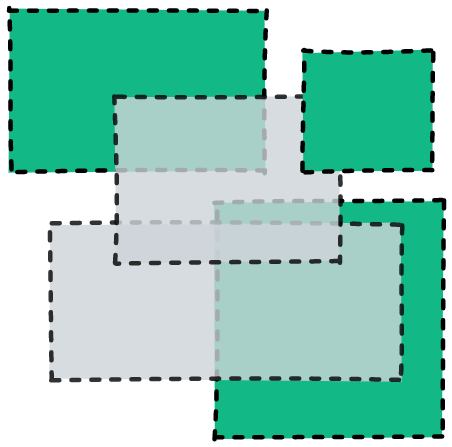
\includegraphics[height=0.3\textheight]{misr.png}
    \end{center}
    }
\end{frame}

\begin{frame}{Maximum Independent Set of Rectangles}
    \begin{fakt}[Marx, ESA '05]
        MISR is $W[1]$-hard by reduction from Clique problem known to be $W[1]$-complete.
    \end{fakt}
    Hence, there is no FPT algorithm for MISR.
    \begin{thm}[PAS for MISR]
        There is a PAS for MISR with running time $k^{\bigO(k/\varepsilon^8)}n^{\bigO(1/\varepsilon^8)}.$
    \end{thm}
\end{frame}

\begin{frame}{Maximum Independent Set of Rectangles}
    \visible<1->{
    \begin{minipage}{0.5\textwidth}
    \begin{block}{Grid}
    \begin{itemize}
        \item<1-> non-uniform
        
        \item<2-> $k$ columns
        
        \item<3-> $k$ rows
        
        \item<4-> each input rectangle overlaps a corner of grid
    \end{itemize} 
    \end{block}
    \end{minipage}\hfill
    \begin{minipage}{0.4\textwidth}
        \begin{center} 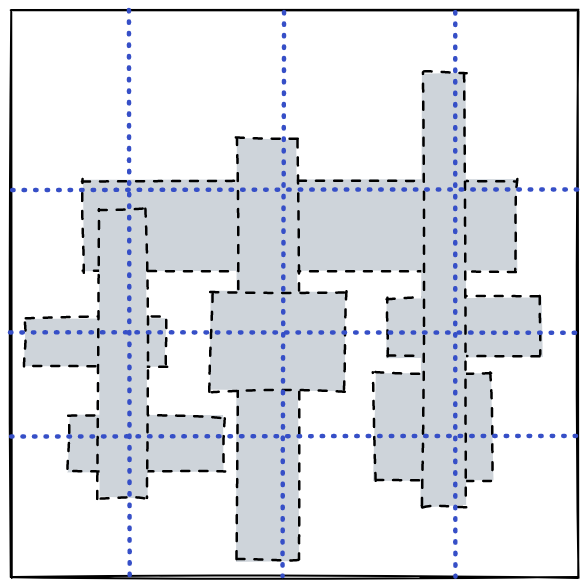
\includegraphics[width=\textwidth]{grid.png}
        \end{center}
    \end{minipage}
    }
\end{frame}

\begin{frame}{Maximum Independent Set of Rectangles}
    \visible<1->{
    \begin{minipage}{0.5\textwidth}
    \begin{block}{Grid}
    \begin{itemize}
        \item<1-> $k - 1$ vertical lines
        % \pause
        \item<2-> $k - 1$ horizontal lines
        % \pause
        \item<3-> each input rectangle intersects horizontal and vertical line
    \end{itemize}
    \end{block}
    \end{minipage}\hfill
    \begin{minipage}{0.4\textwidth}
        \begin{center}
            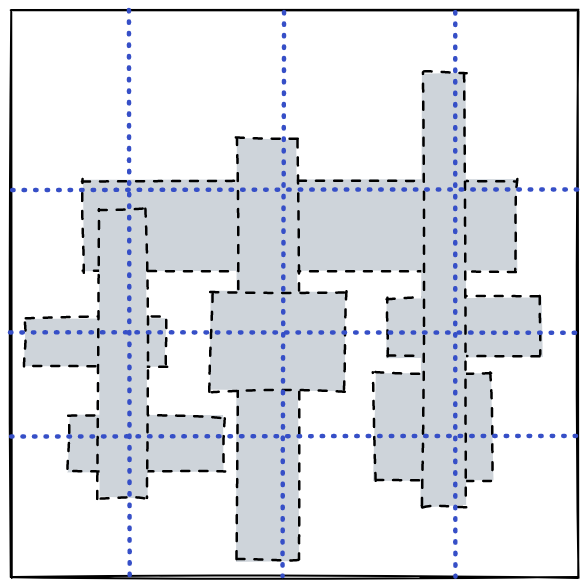
\includegraphics[width=\textwidth]{grid.png}
        \end{center}
    \end{minipage}
    }
\end{frame}

\begin{frame}{Maximum Independent Set of Rectangles}
    \begin{lm}
        There is a polynomial time algorithm such that: 
        \pause
        \begin{itemize}
            \item it computes a set of at most $k - 1$ vertical lines $\mathcal{L}_V$
            \pause
            \item each input rectangle is crossed by a computed line
        \end{itemize}
        or
        \pause
        \begin{itemize}
        
            \item it computes a feasible solution with $k$ rectangles.
        \end{itemize}
        \pause
        Same statement holds for horizontal lines.
    \end{lm}
\end{frame}

\begin{frame}{Maximum Independent Set of Rectangles}
    \begin{minipage}{0.45\textwidth}
        
        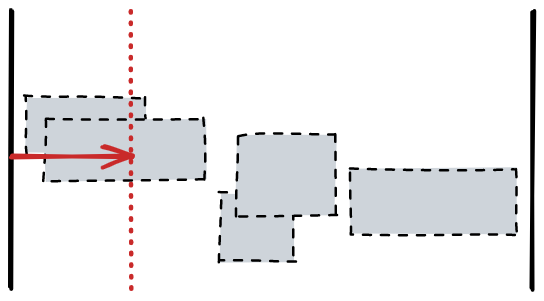
\includegraphics[width=\textwidth]{l1c1.png}
    \end{minipage}\hfill
    \begin{minipage}{0.45\textwidth}
        \begin{center}
            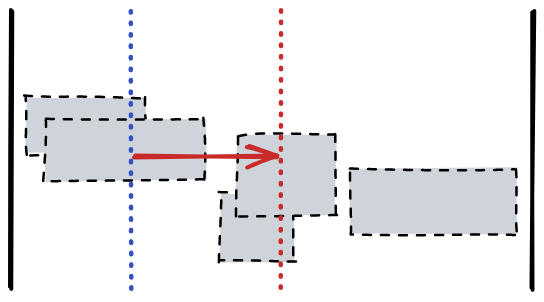
\includegraphics[width=\textwidth]{l1c2.png}
        \end{center}
    \end{minipage}
\end{frame}

\begin{frame}{Maximum Independent Set of Rectangles}
    \begin{minipage}{0.45\textwidth}
        
        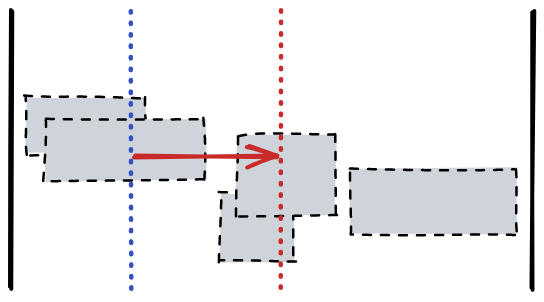
\includegraphics[width=\textwidth]{l1c2.png}
    \end{minipage}\hfill
    \begin{minipage}{0.45\textwidth}
        \begin{center}
            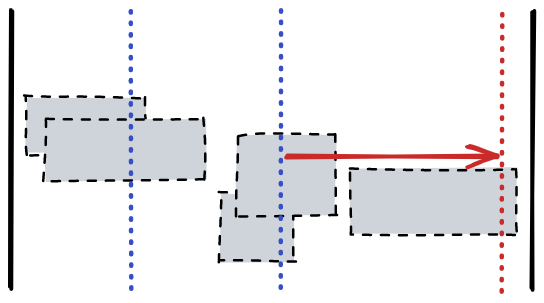
\includegraphics[width=\textwidth]{l1c3.png}
        \end{center}
    \end{minipage}
\end{frame}
\begin{frame}{Maximum Independent Set of Rectangles}
    \begin{minipage}{0.45\textwidth}
        
        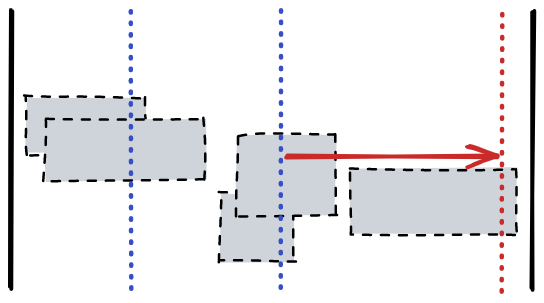
\includegraphics[width=\textwidth]{l1c3.png}
    \end{minipage}\hfill
    \begin{minipage}{0.45\textwidth}
        \begin{center}
            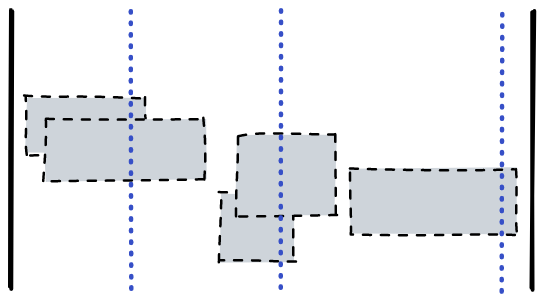
\includegraphics[width=\textwidth]{l1c4.png}
        \end{center}
    \end{minipage}
\end{frame}

\begin{frame}{Maximum Independent Set of Rectangles}
    If we drew less than $k$ lines
    \begin{itemize}
        \item we're done constructing at most $k - 1$ lines such that each input rectangle is intersected by one of these.
    \end{itemize}
    \pause
    else
    \pause
    \begin{itemize}
        \item we can find a rectangle corresponding to each line
        \pause
        \item coordinates of rectangles are integer, so by construction, any pair of rectangles corresponding to two different lines is disjoint
        \pause
        \item chosen rectangles are pairwise disjoint thus form a feasible solution.
        \pause
    \end{itemize}
    Identical arguments apply to horizontal lines.
\end{frame}

\begin{frame}{Maximum Independent Set of Rectangles}
    Applying the lemma, we either 
    \begin{itemize}
        \pause
        \item find a set of $k$ independent rectangles
    \end{itemize} 
    \pause
    or
    \begin{itemize}
        \pause
        \item obtain $\mathcal L_{V}$ and $\mathcal L _{H}.$
    \end{itemize}
    \pause
    For convenience, we define edge lines for both sets, so
    $$
        \mathcal L_V = \mathcal L_V \cup \left\{\ell_0^V = 0, \ell_{|\mathcal L_V| + 1}^V = 2n - 1\right\}
    $$
    \pause
    $$
        \mathcal L_H = \mathcal L_H \cup \left\{\ell_0^H = 0, \ell_{|\mathcal L_H| + 1}^H = 2n - 1\right\}
    $$
\end{frame}

\begin{frame}{Maximum Independent Set of Rectangles}
    \visible<1->{
    \begin{minipage}{0.6\textwidth}
    \begin{block}{Grid cell}
        \begin{itemize}
            \item<1-> two consecutive vertical lines $\ell_i^V, \ell_{i+1}^V$;
            % \pause
            \item<2-> two consecutive horizontal lines $\ell_j^H, \ell_{j+1}^H;$
            % \pause
            \item<3-> cell's corners are the intersection of these lines;
            % \pause
            \item<4-> we interpret cell as a closed set;
            % \pause
            \item<5-> we denote the set of grid cells by $\mathcal G.$
        \end{itemize}
    \end{block}    
    \end{minipage}\hfill
    % \pause
    \begin{minipage}{0.35\textwidth}
    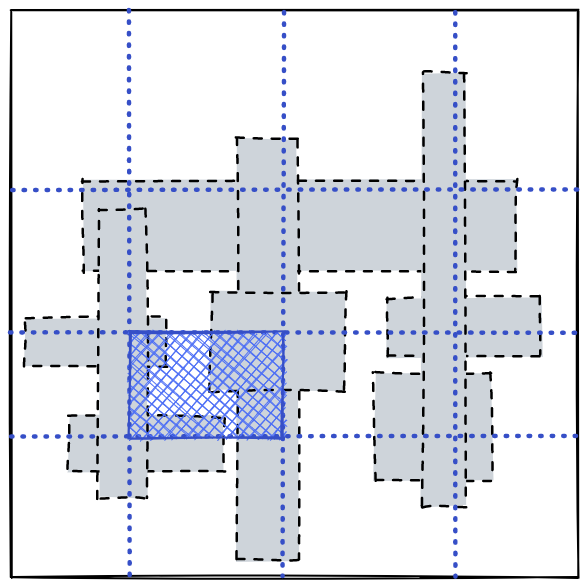
\includegraphics[width=\textwidth]{cell.png}
    \end{minipage}
    }
\end{frame}

\begin{frame}{Maximum Independent Set of Rectangles}
    \visible<1->{
    \begin{minipage}{0.5\textwidth}
        \visible<1->{Define $\mathcal G(R)$ as a rectangle of cells intersected by $R.$} \\
        % \pause
        \visible<2->{Each $\mathcal G(R)$ can be specified by its corner cells, so there are at most $k^4$ choices of $\mathcal G(R)$ for each $R.$}
        % \pause
        \visible<3->{
        \begin{fakt}
            \label{corners}
            It takes $k^{\bigO(k)}$ time to guess the set of grid corners contained in $R$ for each $R$ from solution.
        \end{fakt}}
    \end{minipage}\hfill
    \begin{minipage}{0.4\textwidth}
        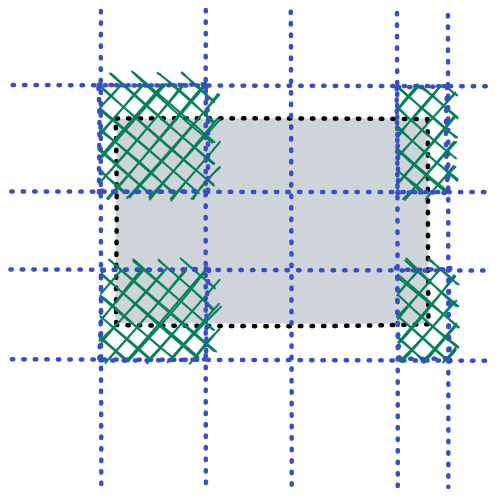
\includegraphics[width=\textwidth]{l14.png}
    \end{minipage}
    }
    
\end{frame}

\begin{frame}{Maximum Independent Set of Rectangles}
    \visible<1->{
    \begin{minipage}{0.55\textwidth}
        \begin{block}{Graph $G_1$}
        \begin{itemize}
            \item<1-> $G_1 = (\mathcal R^*, E_1)$ for given solution $\mathcal R^*;$
            % \pause
            
            \item<2-> $(R_i, R_j) \in E_1$ if and only if there exists such $g \in \mathcal G$ that $R_i$ and $R_j$ intersect $g$ and are adjacent in other than anti-diagonal way in $g.$
        \end{itemize}
    \end{block}
    \end{minipage}\hfill
    \begin{minipage}{0.35\textwidth}
        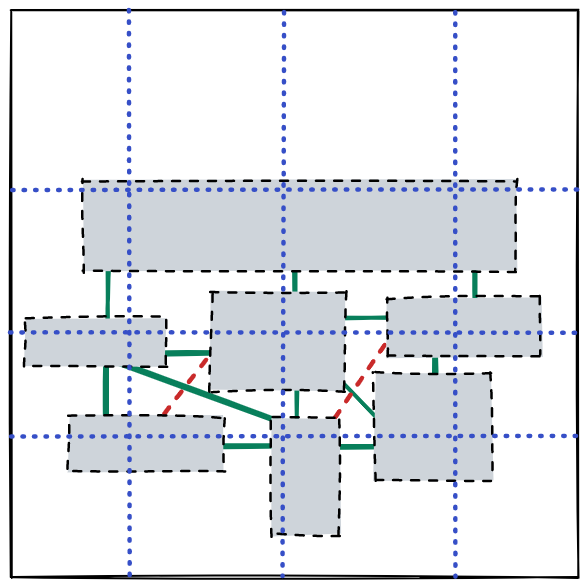
\includegraphics[width=\textwidth]{g12.png}
    \end{minipage}
    }
    
\end{frame}

\begin{frame}{Maximum Independent Set of Rectangles}
    \begin{minipage}{0.45\textwidth}
    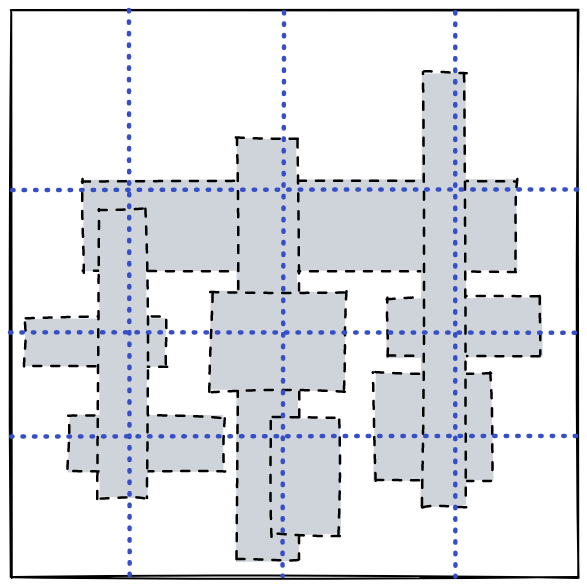
\includegraphics[width=\textwidth]{g11.png}
    \end{minipage}\hfill
    % \pause
    \begin{minipage}{0.45\textwidth}
    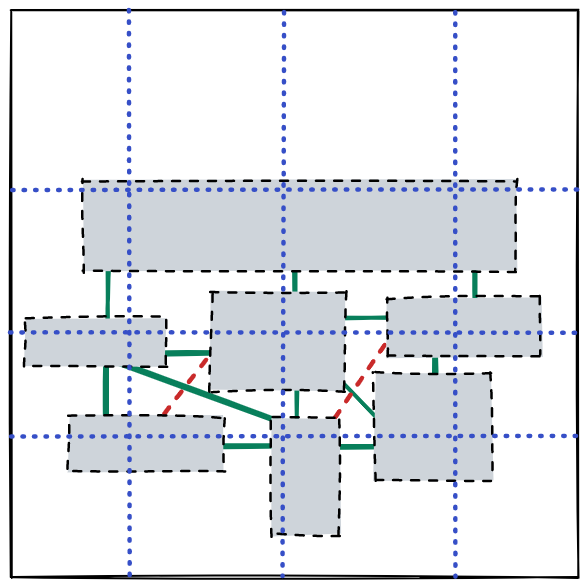
\includegraphics[width=\textwidth]{g12.png}
    \end{minipage}
\end{frame}

\begin{frame}{Maximum Independent Set of Rectangles}
    \visible<1->{
    \begin{minipage}{0.55\textwidth}
        We draw edges in $G_1$ as:
        \visible<2->{
            \begin{itemize}
                \item segments included in grid lines
            \end{itemize}}
        \visible<3->{or}
        \visible<4-> {
            \begin{itemize}
                \item diagonals of cells.
            \end{itemize}}
        \visible<5->{Hence}
        \visible<6->{
            \begin{lm}
                The graph $G_1$ is planar.
            \end{lm}}
    \end{minipage}\hfill
    \begin{minipage}{0.35\textwidth}
        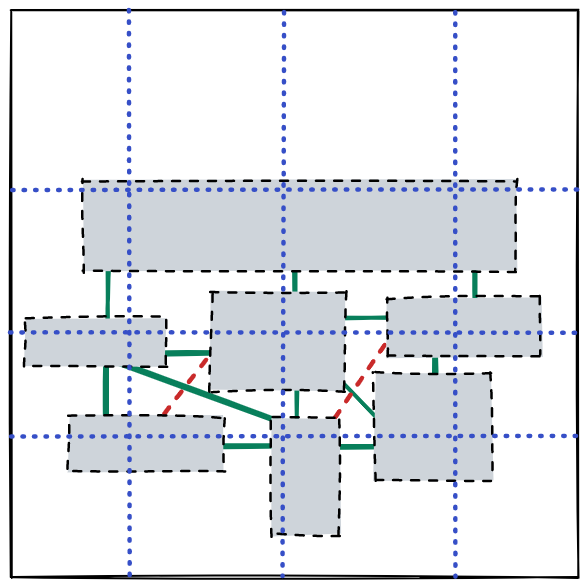
\includegraphics[width=\textwidth]{g12.png}
    \end{minipage}}
    
\end{frame}

\begin{frame}{Maximum Independent Set of Rectangles}
    \begin{minipage}{0.45\textwidth}
    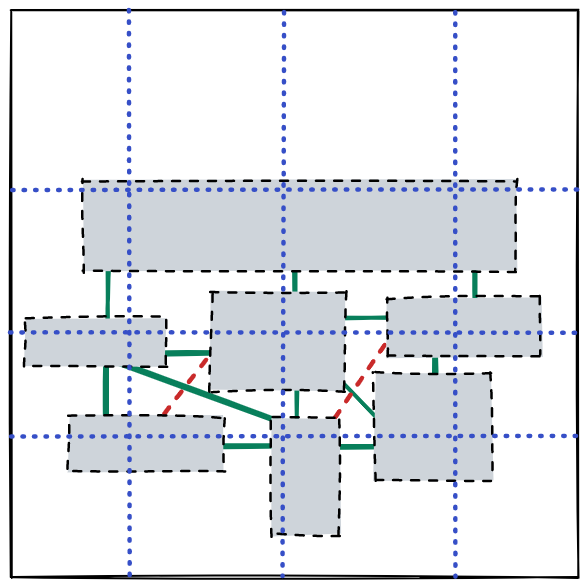
\includegraphics[width=\textwidth]{g12.png}
    \end{minipage}\hfill
    % \pause
    \begin{minipage}{0.45\textwidth}
    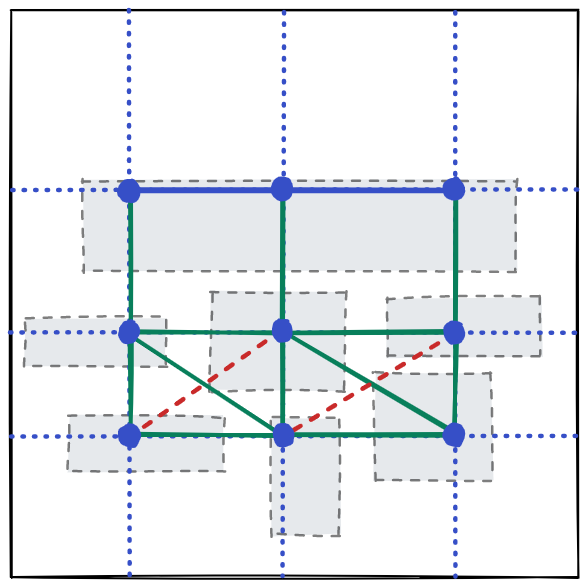
\includegraphics[width=\textwidth]{g13.png}
    \end{minipage}
\end{frame}

\begin{frame}{Maximum Independent Set of Rectangles}
    \visible<1->{
    \begin{lm}
    \label{lemma9}
        Let
        \begin{itemize}
            \item<1-> $G = (V, E)$ is a planar graph
            \item<1-> $\varepsilon' > 0.$
        \end{itemize}
        % \pause
        \visible<2->{There exists a value $c' = \bigO(1/(\varepsilon')^2)$ for which:}
        \begin{itemize}
            \item<3-> there is $V' \subseteq V$ with $|V'| \geqslant (1-\varepsilon')|V|$
            % \pause
            \item<4-> in the graph $G' = G[V']$ each connected component has at most $c'$ vertices.
        \end{itemize}
    \end{lm}
    \begin{center}
        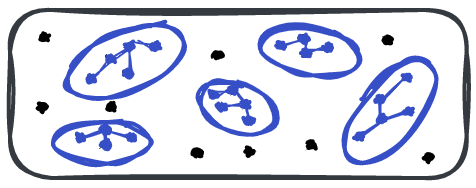
\includegraphics[width=0.5\textwidth]{l3.png}
    \end{center}
    }
\end{frame}

\begin{frame}{Maximum Independent Set of Rectangles}
    \begin{fakt}[Federickson]
     For any integer $r$ any $n$-vertex planar graph can be divided into $\bigO(n/r)$ regions with no more than $r$ vertices each, and $\bigO(n/\sqrt r)$ boundary vertices in total.
    \end{fakt}
    \pause
    We fix $r = \bigO(1/(\varepsilon')^2)$ and then we have at most $\varepsilon' \cdot n$ boundary vertices in total. We define $V'$ to be the set of non-boundary vertices. That proves above lemma.
\end{frame}

\begin{frame}{Maximum Independent Set of Rectangles}
    \begin{block}{Graph $G_1'$}
        \begin{itemize}
            \item set $\varepsilon' = \varepsilon/2;$
            \pause
            \item let $c_1 = \bigO(1/\varepsilon^2);$
            \pause
            \item apply lemma \ref{lemma9} to $G_1$ with respective values.
        \end{itemize}
    \end{block}
\end{frame}

\begin{frame}{Maximum Independent Set of Rectangles}
    \visible<1->{
    \begin{minipage}{0.55\textwidth}
        \begin{block}{Graph $G_2$}
        \begin{itemize}
            \item<1-> $G_2 = (V_2, E_2);$
            % \pause
            \item<2-> $v \in V_2$ represents one connected component in $G_1';$
            % \pause
            \item<3-> there is an edge connecting $w_i, w_j \in V_2$ if there are $R_i, R_j$ such that:
            % \pause
            \begin{itemize}
                \item<4-> they belong to the respective connected components of $G_1';$ 
                % \pause
                \item<5-> there is such a grid cell $g \in \mathcal G$ that $R_i$ and $R_j$ adjacent diagonally in $g.$
            \end{itemize}
        \end{itemize}
    \end{block}
    \end{minipage}\hfill
    \begin{minipage}{0.35\textwidth}
        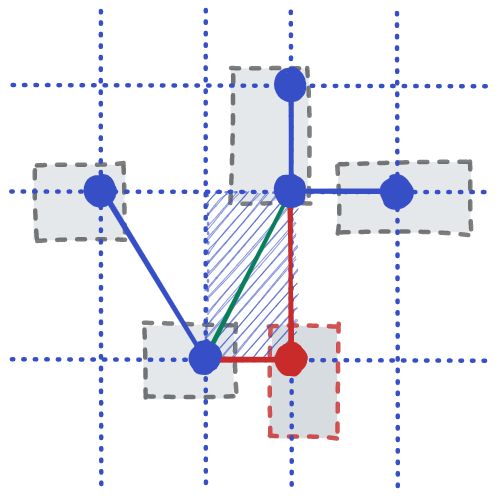
\includegraphics[width=\textwidth]{g22.png}
    \end{minipage}
    }
    
\end{frame}

\begin{frame}{Maximum Independent Set of Rectangles}
    \begin{minipage}{0.45\textwidth}
    \begin{lm}
        Graph $G_2$ is planar.
    \end{lm}
    \end{minipage}\hfill
    \begin{minipage}{0.45\textwidth}
    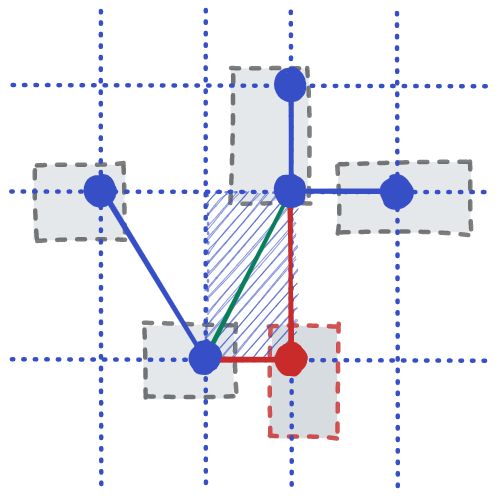
\includegraphics[width=\textwidth]{g22.png}
    \end{minipage}
\end{frame}

\begin{frame}{Maximum Independent Set of Rectangles}
    \begin{block}{Graph $G_2'$}
    \begin{itemize}
        \item set $\varepsilon' = \varepsilon/2c_1;$
        \pause
        \item let $c_2 = \bigO((1/\varepsilon')^2) = \bigO(1/\varepsilon^6);$
        \pause
        \item apply lemma \ref{lemma9} to $G_2$ with respective values.
    \end{itemize}
    \end{block}
\end{frame}

\begin{frame}{Maximum Independent Set of Rectangles}
    \visible<1->{
    \begin{minipage}{0.5\textwidth}
    We define a group $\mathcal R_q'$ for each connected component $\mathcal C_q$ of $V_2'.$ \\
    % \pause
    \visible<2->{The set $\mathcal R_q'$ contains all rectangles contained in the connected component $\mathcal C_q$ of $V_2'.$}
    \end{minipage}\hfill
    % \pause
    \begin{minipage}{0.4\textwidth}
        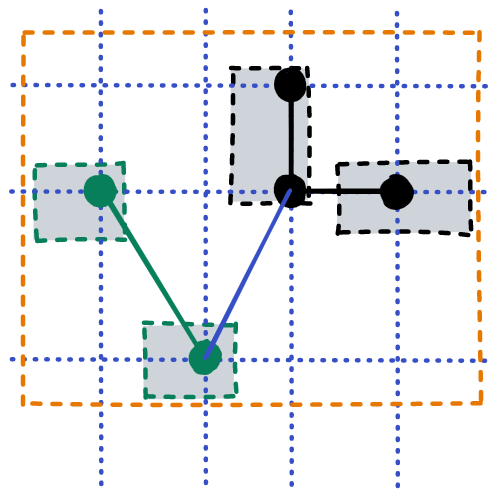
\includegraphics[width=\textwidth]{rq.png}
    \end{minipage} \\}
    \visible<3->{
    We define $\mathcal R' = \coprod_q \mathcal R_q'.$}
    
\end{frame}

\begin{frame}{Maximum Independent Set of Rectangles}
    \begin{minipage}{0.5\textwidth}
    \begin{lm}
        \label{lemma11}
        If $R_i, R_j \in \mathcal R'$ intersect the same cell $g \in \mathcal G,$ then there is such $\mathcal R_q'$ that $R_i, R_j \in \mathcal R_q'.$
    \end{lm}
    \end{minipage}\hfill
    \begin{minipage}{0.4\textwidth}
        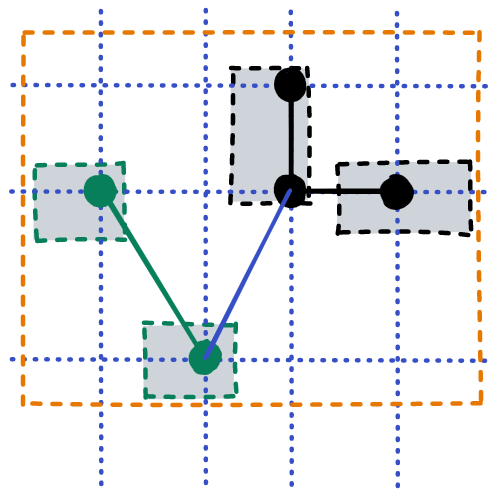
\includegraphics[width=\textwidth]{rq.png}
    \end{minipage} \\
\end{frame}

\begin{frame}{Maximum Independent Set of Rectangles}
    \begin{minipage}{0.45\textwidth}
    \begin{block}{Graph $G_1'$}
        \begin{itemize}
            \item set $\varepsilon' = \varepsilon/2;$
            \item let $c_1 = \bigO(1/\varepsilon^2);$
            \item apply lemma \ref{lemma9} to $G_1$ with respective values.
        \end{itemize} 
    \end{block}
    \pause
        Component $C_i$ of $G_1'$ contains at most $c_1 = \bigO(1/\varepsilon^2)$ vertices.
    \end{minipage}\hfill
    \begin{minipage}{0.45\textwidth}
        \begin{block}{Graph $G_2'$}
    \begin{itemize}
        \item set $\varepsilon' = \varepsilon/2c_1;$
        \item let $c_2 = \bigO((1/\varepsilon')^2) = \bigO(1/\varepsilon^6);$
        \item apply lemma \ref{lemma9} to $G_2$ with respective values.
    \end{itemize}
    \end{block}
    \pause
    Component $\mathcal C_i$ of $G_2'$ contains at most $c_2 = \bigO(1/\varepsilon^6)$ vertices. 
    \end{minipage}
    \pause
    \begin{lm}
        \label{lemma12}
        There is a constant $c = \bigO(1/\varepsilon^8)$ such that for each group $|\mathcal R_q'| \leqslant c.$
    \end{lm}
\end{frame}

\begin{frame}{Maximum Independent Set of Rectangles}
    \begin{lm}
        \label{lemma13}
        $|\mathcal R'| \geqslant (1 - \varepsilon)|\mathcal R^*|.$
    \end{lm}
    \pause
    \begin{itemize}
        \item at most $|V_1| \cdot \frac\varepsilon2$ vertices are deleted from $G_1$ constructing $G_1'$
        \pause
        \item at most $|V_2| \cdot \frac{\varepsilon}{2c_1}$ vertices are deleted while constructing $G_2'$
        \pause
        \item Deleted vertices from $V_2$ represent at most $c_1 \cdot \frac{\varepsilon}{2c_1}|V_2| \leqslant |V_1'|\cdot \varepsilon/2 \leqslant |V_1| \cdot \varepsilon/2$ in $G_1$
        \pause
        \item $|\mathcal R'| \geqslant |\mathcal R^*| - 2 \cdot \frac{\varepsilon}{2}|V_1| = (1 - \varepsilon)|\mathcal R^*|.$
    \end{itemize}
\end{frame}

\begin{frame}{Maximum Independent Set of Rectangles}
    \visible<1->{We have finally gathered all tools to prove the following}
    \visible<2->{
    \begin{minipage}{0.55\textwidth}
        \begin{lm}
        \label{lemma7}
        Let $|R^*| = k$ be the solution to the given instance. There is a constant $c = \bigO(1/\varepsilon^8)$ such that:
        \pause
        \begin{itemize}
            \item<3-> there is a solution $\mathcal R' \subseteq \mathcal R^*;$
            % \pause
            \item<4-> $|\mathcal R'| \geqslant (1 - \varepsilon) |\mathcal R^*|;$
            % \pause
            \item<5-> $\coprod_{i=1}^s \mathcal R_i'$ with $s \leqslant k;$
            % \pause
            \item<6-> $|\mathcal R_j'| \leqslant c$
            for $1\leqslant j \leqslant s;$
            % \pause
            \item<7-> if $R_i, R_j \in \mathcal R'$ intersect the same cell $g \in \mathcal G$ then $R_i, R_j \in \mathcal R_t'.$
        \end{itemize}
    \end{lm}
    \end{minipage}\hfill
    \begin{minipage}{0.35\textwidth}
        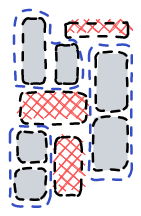
\includegraphics[width=\textwidth]{l8.png}
    \end{minipage}
    }
    
\end{frame}

\begin{frame}{Maximum Independent Set of Rectangles}
    Let $\mathcal G_j$ be the set of cells intersected by at least one rectangle from $\mathcal R_j'.$ \\
    \pause
    By constructions, each cell can be intersected by rectangles of at most one group so they are disjoint. \\
\end{frame}

\begin{frame}{Maximum Independent Set of Rectangles}
    \visible<1->{
    \begin{minipage}{0.55\textwidth}
    \begin{itemize}
        \item<1->{$\mathcal G_j = \bigcup_{R \in \mathcal R_j} \mathcal G(R).$}
        % \pause
        \item<2->{By lemma \ref{lemma7}, $|\mathcal R_j'| \leqslant c = \bigO(1/\varepsilon^8).$}
    \end{itemize}
        % \pause
        \visible<3->{From fact \ref{corners}}
        \visible<4->{
        \begin{lm}
            Each $\mathcal G_j$ can be computed in polynomial time $k^{\bigO(1/\varepsilon^8)}$.
        \end{lm}}
    \end{minipage}\hfill
    \begin{minipage}{0.4\textwidth}
        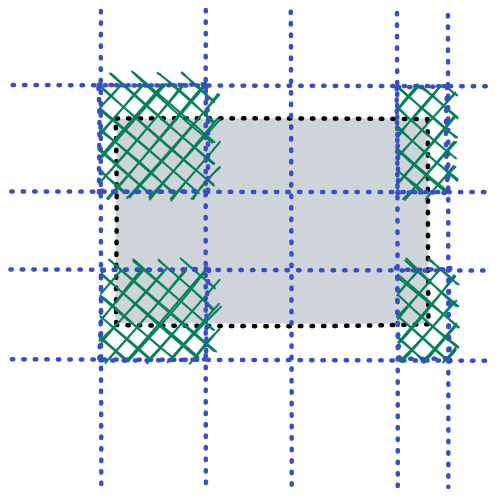
\includegraphics[width=\textwidth]{l14.png}
    \end{minipage}
    }
\end{frame}

\begin{frame}{Maximum Independent Set of Rectangles}
    \begin{thm*}[PAS for MISR]
        There is a PAS for MISR with running time $k^{\bigO(k/\varepsilon^8)}n^{\bigO(1/\varepsilon^8)}.$
    \end{thm*}
\end{frame}

\begin{frame}{The end}
    \centerline{Thank you!}
\end{frame}

% \AtBeginSection[ ]
% {
% \begin{frame}{Outline}
    % \/tableofcontents[currentsection]
% \end{fra/me}
% }

%\AtBeginSubsection[ ]
%{
%\begin{frame}{Outline}
%    \tableofcontents[currentsection]
%\end{frame}
%}

% \AtBeginSubsection[]{
%   \frame<beamer>{ 
    % \frametitle{Outline}   
% 
% \tableofcontents[currentsection,currentsubsection,sectionstyle=show,subsectionstyle=show/shaded,]}
% }



\end{document} 